\documentclass[final]{beamer}

\usepackage[scale=1.24]{beamerposter} % Use the beamerposter package for laying out the poster

\usepackage{siunitx}

\usetheme{confposter} % Use the confposter theme supplied with this template

\setbeamercolor{block title}{fg=nblue,bg=white} % Colors of the block titles
\setbeamercolor{block body}{fg=black,bg=white} % Colors of the body of blocks
\setbeamercolor{block alerted title}{fg=white,bg=dblue!70} % Colors of the highlighted block titles
\setbeamercolor{block alerted body}{fg=black,bg=dblue!10} % Colors of the body of highlighted blocks
% Many more colors are available for use in beamerthemeconfposter.sty

\usepackage[skins]{tcolorbox}
% a "sub-block" (plain block-within-block (second-level header))
\newenvironment{subblock}[1]{
  \setbeamertemplate{block begin}
  {
    \setbeamercolor{block title}{fg=nblue!90} % @TODO defer to beamercolortheme
    \par\vskip\medskipamount
    \begin{beamercolorbox}[colsep*=0ex,dp={2ex}]{block title}
      \vskip-0.5cm
      \begin{tikzpicture}[every node/.style={inner sep=0}]
        \node (titlenode) at (0.1cm, 0) {\usebeamerfont{block title}\normalsize\insertblocktitle};
        \tcbsetmacrotowidthofnode{\titlewidth}{titlenode}
        \tcbsetmacrotoheightofnode{\titleheight}{titlenode}
        \shade [inner color=nblue!16!black!24,outer color=white]
        (-\titlewidth/2,-\titleheight/2) rectangle ++({1.1*\titlewidth+0.1cm},-0.2cm);
      \end{tikzpicture}
    \end{beamercolorbox}
    {\parskip0pt\par}
    \ifbeamercolorempty[bg]{block title}
    {}
    {\ifbeamercolorempty[bg]{block body}{}{\nointerlineskip\vskip-0.5pt}}
    \usebeamerfont{block body}
    \vskip-0.5cm
    \begin{beamercolorbox}[colsep*=0ex,vmode]{block body}
      \justifying
    }
    \setbeamertemplate{block end}
    {
    \end{beamercolorbox}
    \vskip\smallskipamount
  }
  \begin{block}{{\normalsize #1}}
  }{\end{block}}

\newlength{\sepwid}
\newlength{\colonewid}
\newlength{\coltwowid}
\newlength{\colthreewid}
\setlength{\paperwidth}{48in} % A0 width: 46.8in
\setlength{\paperheight}{36in} % A0 height: 33.1in
\setlength{\sepwid}{0.024\paperwidth} % Separation width (white space) between columns
\setlength{\colonewid}{0.29\paperwidth} % Width of column one
\setlength{\coltwowid}{0.31\paperwidth} % Width of column two
\setlength{\colthreewid}{0.30\paperwidth} % Width of one column
\setlength{\topmargin}{-0.5in} % Reduce the top margin size
% -----------------------------------------------------------

\usepackage{graphicx}  % Required for including images
\usepackage{booktabs} % Top and bottom rules for tables
\usepackage{tikz}
\usetikzlibrary{
  arrows,
  calc,
  decorations.pathmorphing,
  decorations.pathreplacing,
  decorations.markings,
  fadings,
  positioning,
  shapes,
  arrows.meta
}
\usepgfmodule{oo}

\pgfdeclareradialshading{glow2}{\pgfpoint{0cm}{0cm}}{
  color(0mm)=(white);
  color(2mm)=(white);
  color(8mm)=(black);
  color(10mm)=(black)
}
\pgfdeclareradialshading{glow}{\pgfpoint{0cm}{0cm}}{
  color(0mm)=(white);
  color(5mm)=(white);
  color(9mm)=(black);
  color(10mm)=(black)
}

\begin{tikzfadingfrompicture}[name=glow fading]
  \shade [shading=glow] (0,0) circle (1);
\end{tikzfadingfrompicture}

\begin{tikzfadingfrompicture}[name=glow2 fading]
  \shade [shading=glow2] (0,0) circle (1);
\end{tikzfadingfrompicture}

\definecolor{atomorange}{rgb}{1.0,0.483,0.0}
\definecolor{pyplotc0}{rgb}{0.122,0.467,0.706}
\definecolor{pyplotc1}{rgb}{1.000,0.498,0.055}
\definecolor{pyplotc2}{rgb}{0.173,0.627,0.173}
\definecolor{pyplotc3}{rgb}{0.839,0.153,0.157}
\definecolor{pyplotc4}{rgb}{0.580,0.404,0.741}
\definecolor{pyplotc5}{rgb}{0.549,0.337,0.294}
\definecolor{pyplotc6}{rgb}{0.890,0.467,0.761}
\definecolor{pyplotc7}{rgb}{0.498,0.498,0.498}
\definecolor{pyplotc8}{rgb}{0.737,0.741,0.133}
\definecolor{pyplotc9}{rgb}{0.090,0.745,0.812}

\pgfdeclarelayer{tweezer}
\pgfsetlayers{tweezer,main}
\pgfooclass{tweezer}{
  \method tweezer() {
  }
  \method drawTweezer(#1,#2,#3) {
    \shade[shading=radial,path fading=glow fading,shift={(#1,#2)},rotate=90,yscale=1,
    fill opacity=0.9,inner color=#3]
    plot[draw,samples=200,domain=-4.5:4.5] function {sqrt(0.02 + (x)**2 / 10)}
    -- plot[draw,samples=200,domain=4.5:-4.5] function {-sqrt(0.02 + (x)**2 / 10)};
  }
  \method drawRaman(#1,#2) {
    \pgfoothis.drawTweezer(#1,#2,pyplotc4);
  }
  \method drawAtom(#1,#2,#3,#4) {
    \fill [#4,path fading=glow2 fading] (#1,#2) circle (#3);
  }
  \method drawDownAtom(#1,#2,#3) {
    \pgfoothis.drawAtom(#1,#2,#3,pyplotc0);
  }
  \method drawUpAtom(#1,#2,#3) {
    \pgfoothis.drawAtom(#1,#2,#3,pyplotc1);
  }
}
\pgfoonew \mytweezer=new tweezer()



% --------------------------------------------------------------------------------
%	TITLE SECTION
% --------------------------------------------------------------------------------

\def\realtitle{Mid-circuit measurement and reset on $^{171}$Yb$^+$ using the \textit{omg} architecture}

\title{%
  \texorpdfstring{%
    \makebox[\linewidth]{%
      \makebox[0pt][l]{%
        \raisebox{\dimexpr-\height+0.5\baselineskip}[0pt][0pt]
        {
          \begin{tikzpicture}
            \node at (0, 0) {
\includegraphics[width=20cm]{imgs/logos/Duke}};
            \node at (-4, -4) {
\includegraphics[width=6.5cm]{imgs/logos/Sandia}};
          \end{tikzpicture}
        }% Left logo
      }\hfill
      \makebox[0pt]{\textcolor{dblue}{\realtitle}}%
      \hfill\makebox[0pt][r]{%
        \raisebox{\dimexpr-\height+0.5\baselineskip}[0pt][0pt]
        {
          \begin{tikzpicture}
            \node at (0, 0) {
\includegraphics[width=16cm]{imgs/logos/QSA}};
            \node at (11, 0) {\includegraphics[width=4cm]{imgs/logos/DoE}};
            % DARPA
            % IARPA
            \node at (11, -4.3) {
\includegraphics[width=4cm]{imgs/logos/ARL}};
            \node at (-6, -4.3) {\includegraphics[width=4cm]{imgs/logos/NSF}};
            \node at (0, -4.3) {\includegraphics[width=6cm]{imgs/logos/DARPA}};
            \node at (6, -4) {
\includegraphics[width=4.5cm]{imgs/logos/IARPA}};
          \end{tikzpicture}
        }% Right logo
      }%
    }%
  }
  {\realtitle}} % Poster title

\author{Yichao Yu, Keqin Yan, Debopriyo Biswas,
  Vivian Zhang, Bahaa Harraz,\\
  Marko Cetina, Crystal Noel, Alexander Kozhanov,
  Christopher R Monroe}
\institute{Duke Quantum Center, Duke University}

\ifpdf
  % Ensure reproducible output
  \pdfinfoomitdate=1
  \pdfsuppressptexinfo=-1
  \pdftrailerid{}
  \hypersetup{
    pdfcreator={},
    pdfproducer={}
  }
\fi

\begin{document}

\addtobeamertemplate{block end}{}{\vspace*{2ex}} % White space under blocks
\addtobeamertemplate{block alerted end}{}{\vspace*{2ex}} % White space under highlighted (alert) blocks

\setlength{\belowcaptionskip}{2ex} % White space under figures
\setlength\belowdisplayshortskip{2ex} % White space under equations

\definecolor{trapyellow}{HTML}{ffe0a5}
\definecolor{semgray}{HTML}{cccccc}

\begin{frame}[t] % The whole poster is enclosed in one beamer frame
  \begin{columns}[t]
    \begin{column}{\sepwid}\end{column} % Empty spacer column
    \begin{column}{\colonewid} % The first column
      % First column
      % Mid-circuit measurement
      % OMG
      % System
      \begin{block}{Mid-circuit measurement and reset (MCMR) and the \textit{omg} architecture}
        \begin{center}
          \begin{subblock}{MCMR}
            \begin{columns}
              \begin{column}{0.38\colonewid}
                \begin{itemize}
                \item Required for multiple rounds of error correction
                \item Partial readout without perturbing the rest of the system
                \item Partial reset for qubit reuse
                \end{itemize}
              \end{column}
              \begin{column}{0.58\colonewid}
                \begin{tikzpicture}
                  \node[rotate=90] (I) at (0, 0) {Logical qubits};
                  \node[align=center,draw,minimum height=4cm] (M) at (5, 0) {Stabilizer\\measurement};
                  \node[align=center,draw,minimum height=4cm] (C) at (13, 0) {Correction};
                  \draw (I) -- (M);
                  \draw ($(I.south) + (0, 1)$) -- ($(M.west) + (0, 1)$);
                  \draw ($(I.south) + (0, -1)$) -- ($(M.west) + (0, -1)$);

                  \draw (M) -- (C);
                  \draw ($(M.east) + (0, 1)$) -- ($(C.west) + (0, 1)$);
                  \draw ($(M.east) + (0, -1)$) -- ($(C.west) + (0, -1)$);

                  \draw ($(C.east) + (0, 1)$) -- ++(2, 0);
                  \draw ($(C.east) + (0, 0)$) -- ++(2, 0);
                  \draw ($(C.east) + (0, -1)$) -- ++(2, 0);

                  \draw[-{Stealth[length=6mm,width=4.5mm]},line width=4] (M.south) -- (5, -3) -- node[below] {Feedback} (13, -3) -- (C.south);
                \end{tikzpicture}
              \end{column}
            \end{columns}
          \end{subblock}
          \vspace{1cm}
          \begin{subblock}{\textit{omg} architecture}
            \begin{columns}
              \begin{column}{0.42\colonewid}
                \begin{itemize}
                \item Combining \textbf{\textit{O}}ptical \textbf{\textit{M}}etastable
                  and \textbf{\textit{G}}round state qubits
                  {\scriptsize (Appl. Phys. Lett. 119, 214002 (2021))}
                \item Protecting quantum information by converting between qubit types
                \item Faster than ion-shuttling
                \end{itemize}
              \end{column}
              \begin{column}{0.53\colonewid}
                \begin{itemize}
                \item Yb$^+$: D$_{3/2}$ ($50$ ms), D$_{5/2}$ ($7$ ms),\\
                  \hspace{2.5cm}F$_{7/2}$ ($>1$ yr)
                \item Ba$^+$: D$_{3/2}$ ($20$ s), D$_{5/2}$ ($30$ s)
                \item $\cdots$
                \end{itemize}
              \end{column}
            \end{columns}
            \vspace{0.2cm}
            \begin{center}
              \begin{tikzpicture}[scale=1]
                % P1/2
                \begin{scope}[shift={(0, 15)}]
                  % F=1
                  \draw[line width=2] (-1.8, 1.5) -- (-0.8, 1.5);
                  \draw[line width=2] (-0.5, 1.5) -- (0.5, 1.5);
                  \draw[line width=2] (0.8, 1.5) -- (1.8, 1.5);
                  % F=0
                  \draw[line width=2] (-0.5, 0) -- (0.5, 0);

                  \coordinate (P12) at (0, 0.75);

                  \node[left] at (-1.8, 1.5) {\small $F=1$};
                  \node[left] at (-1.8, 0) {\small $F=0$};

                  \node[left] at (-4.5, 0.75) {\small $^2\mathrm{P}_{1/2}$};
                \end{scope}

                % S1/2
                % F=1
                \draw[line width=2] (-1.8, 2) -- (-0.8, 2);
                \draw[line width=2] (-0.5, 2) -- (0.5, 2);
                \draw[line width=2] (0.8, 2) -- (1.8, 2);
                % F=0
                \draw[line width=2] (-0.5, 0) -- (0.5, 0);

                \coordinate (S12) at (0, 1);

                \node[left] at (-1.8, 2) {\small $F=1$};
                \node[left] at (-1.8, 0) {\small $F=0$};

                \node[left] at (-4.5, 1) {\small $^2\mathrm{S}_{1/2}$};

                % D3/2
                \begin{scope}[shift={(6.5, 7)}]
                  % F=2
                  \draw[line width=2] (-3.1, 1.2) -- (-2.1, 1.2);
                  \draw[line width=2] (-1.8, 1.2) -- (-0.8, 1.2);
                  \draw[line width=2] (-0.5, 1.2) -- (0.5, 1.2);
                  \draw[line width=2] (0.8, 1.2) -- (1.8, 1.2);
                  \draw[line width=2] (2.1, 1.2) -- (3.1, 1.2);
                  % F=1
                  \draw[line width=2] (-1.8, 0) -- (-0.8, 0);
                  \draw[line width=2] (-0.5, 0) -- (0.5, 0);
                  \draw[line width=2] (0.8, 0) -- (1.8, 0);

                  \coordinate (D32) at (0, 0.6);

                  \node[right] at (3.1, 1.2) {\small $F=2$};
                  \node[right] at (3.1, 0) {\small $F=1$};

                  \node[below right] at (3.1, -0.6) {\small $^2\mathrm{D}_{3/2}$};
                \end{scope}

                % D5/2
                \begin{scope}[shift={(6.5, 13)}]
                  % F=2
                  \draw[line width=2] (-3.1, 1.2) -- (-2.1, 1.2);
                  \draw[line width=2] (-1.8, 1.2) -- (-0.8, 1.2);
                  \draw[line width=2] (-0.5, 1.2) -- (0.5, 1.2);
                  \draw[line width=2] (0.8, 1.2) -- (1.8, 1.2);
                  \draw[line width=2] (2.1, 1.2) -- (3.1, 1.2);
                  % F=3
                  \draw[line width=2] (-4.4, 0) -- (-3.4, 0);
                  \draw[line width=2] (-3.1, 0) -- (-2.1, 0);
                  \draw[line width=2] (-1.8, 0) -- (-0.8, 0);
                  \draw[line width=2] (-0.5, 0) -- (0.5, 0);
                  \draw[line width=2] (0.8, 0) -- (1.8, 0);
                  \draw[line width=2] (2.1, 0) -- (3.1, 0);
                  \draw[line width=2] (3.4, 0) -- (4.4, 0);

                  \coordinate (D52) at (0, 0.6);

                  \node[right] at (4.4, 1.2) {\small $F=2$};
                  \node[right] at (4.4, 0) {\small $F=3$};

                  \node[above right] at (4.4, 1.8) {\small $^2\mathrm{D}_{5/2}$};
                \end{scope}

                % F7/2
                \begin{scope}[shift={(19, 6)}]
                  % F=4
                  \draw[line width=2] (-5.7, 1) -- (-4.7, 1);
                  \draw[line width=2] (-4.4, 1) -- (-3.4, 1);
                  \draw[line width=2] (-3.1, 1) -- (-2.1, 1);
                  \draw[line width=2] (-1.8, 1) -- (-0.8, 1);
                  \draw[line width=2] (-0.5, 1) -- (0.5, 1);
                  \draw[line width=2] (0.8, 1) -- (1.8, 1);
                  \draw[line width=2] (2.1, 1) -- (3.1, 1);
                  \draw[line width=2] (3.4, 1) -- (4.4, 1);
                  \draw[line width=2] (4.7, 1) -- (5.7, 1);
                  % F=3
                  \draw[line width=2] (-4.4, 0) -- (-3.4, 0);
                  \draw[line width=2] (-3.1, 0) -- (-2.1, 0);
                  \draw[line width=2] (-1.8, 0) -- (-0.8, 0);
                  \draw[line width=2] (-0.5, 0) -- (0.5, 0);
                  \draw[line width=2] (0.8, 0) -- (1.8, 0);
                  \draw[line width=2] (2.1, 0) -- (3.1, 0);
                  \draw[line width=2] (3.4, 0) -- (4.4, 0);

                  \coordinate (F72) at (0, 0.6);

                  \node[right] at (5.7, 1) {\small $F=4$};
                  \node[right] at (5.7, 0) {\small $F=3$};

                  \node[right] at (8.4, 0.5) {\small $^2\mathrm{F}_{7/2}$};
                \end{scope}

                \draw[-{Stealth[length=6mm,width=4.5mm]},cyan,line width=2]
                (S12) -- node[above,sloped] {\small $370$~nm} (P12);

                \draw[-{Stealth[length=6mm,width=4.5mm]},blue,line width=2]
                (S12) -- node[below,sloped] {\small $435$~nm} (D32);

                \draw[-{Stealth[length=6mm,width=4.5mm]},blue!60!cyan,line width=2]
                (S12) -- node[above,sloped] {\small $411$~nm} (D52);

                \draw[-{Stealth[length=6mm,width=4.5mm]},red!80!black,line width=2]
                (D52) -- node[above,sloped] {\small $3.4$~$\mu$m} (F72);
              \end{tikzpicture}
            \end{center}
          \end{subblock}
        \end{center}
      \end{block}
      \vspace{-1.6cm}

      \begin{block}{System}
        \begin{center}
          \begin{subblock}{Optical control}
            \begin{columns}
              \column{15cm}
              \begin{itemize}
              \item Global state preparation and detection with $370$~nm
              \item Individually addressible Raman with $355$~nm
              \item Global $435$~nm for exciting to D$_{3/2}$ states
              \item (Planned) Global $411$~nm and $3.4$~$\mu$m for accessing D$_{5/2}$
                and F$_{7/2}$ states
              \end{itemize}
              \column{17.5cm}
              \begin{tikzpicture}
                \node at (0, 0) {\includegraphics[width=17.5cm]{imgs/LabPicture}};
                \node at (-6.7, 6) {
\includegraphics[width=4cm]{imgs/logos/L3Harris}};
              \end{tikzpicture}
            \end{columns}
          \end{subblock}
          \vspace{2cm}
          \begin{subblock}{Phoenix surface trap}
            \begin{columns}
              \column{16cm}
              \includegraphics[width=15.5cm]{imgs/Phoenix}
              \column{16cm}
              \begin{itemize}
              \item Separate loading and quantum region
              \item Fine control of ion position
              \item Low heating rate
              \end{itemize}
            \end{columns}
          \end{subblock}
        \end{center}
      \end{block}
      \vspace{-1.2cm}
    \end{column} % End of the first column

    \begin{column}{\sepwid}
      \begin{center}
        {\color{gray}\rule{3pt}{\textheight}}
      \end{center}
    \end{column} % Empty spacer column

    \begin{column}{\coltwowid}
      \begin{block}{MCMR without individual detection beams}
        \begin{center}
          \begin{tikzpicture}
              \node[left,text width=17cm,align=center] at (0, 0) {
                \begin{itemize}
                \item Two methods based on \textit{omg}-architecture
                  to avoid the need for focused detection beam.
                  \vspace{0.5cm}
                \item \textbf{\textit{Hands-off method}}:
                  \begin{itemize}
                  \item Nominally no perturbation on data
                  \item More sensitive to addressing crosstalk
                  \end{itemize}
                  \vspace{0.5cm}
                \item \textbf{\textit{Shelving method}}:
                  \begin{itemize}
                  \item Better protection of data from detection transition
                  \item Relies on metastable state lifetime and coherence
                  \end{itemize}
                \end{itemize}
              };
            \node[right] at (0, 0) {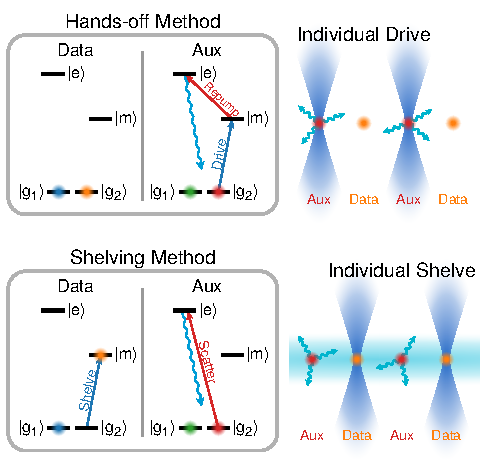
\includegraphics[width=19cm]{imgs/fig-mcmr-methods.pdf}};
          \end{tikzpicture}
        \end{center}
      \end{block}
      \begin{block}{Individual metastable state control}
        \begin{center}
          \vspace{1cm}
          \begin{subblock}{Dressing}
            \begin{tikzpicture}
              \node[left,text width=20cm,align=center] at (0, 6) {
                \begin{itemize}
                \item Use individual beam dressing to shift the metastable state resonance.
                \item Near resonance Raman dressing for $\mathrm{Yb}^+$
                  with $355\ \mathrm{nm}$ due to low scalar light shift.
                \end{itemize}
              };
              \node[left] at (0, -5) {\includegraphics[width=20cm]{imgs/fig-dstate-spec.pdf}};
              \node[text width=15cm,align=center] at (9.5, 3.2) {
                Robust composite pulse for fast preparation of the dressed state
              };
              \node[right] at (0, -4) {\includegraphics[width=16cm]{imgs/fig-dress-rotate.pdf}};
            \end{tikzpicture}
          \end{subblock}
          \vspace{1cm}
          \begin{subblock}{Qubit rotation}
            \begin{tikzpicture}
              \node[text width=26cm,align=left] at (-6, 9) {
                \begin{itemize}
                \item Treat individual shelving as single qudit operation
                \item Realize arbitrary qudit operation with
                  (individual~Raman)~qubit~rotation and global drive to metastable state
                \end{itemize}
              };
              \node at (0, 5) {Example sequence};
              \node at (0, 0) {\includegraphics[width=38cm]{imgs/fig-qubit-rotation.pdf}};
            \end{tikzpicture}
          \end{subblock}
        \end{center}
      \end{block}
    \end{column} % End of the second column

    \begin{column}{\sepwid}
      \begin{center}
        {\color{gray}\rule{3pt}{\textheight}}
      \end{center}
    \end{column} % Empty spacer column

    \begin{column}{\colthreewid} % The third column
      \begin{block}{Results}
        \vspace{0.2cm}
        \begin{center}
          \begin{subblock}{Mid-circuit measurement}
            \begin{center}
              \begin{tikzpicture}
                \node at (0, 0) {\includegraphics[width=27.0cm]{imgs/measure_sequence.pdf}};
                \node[below,text width=18cm,align=left] at (-9, -3) {
                  \begin{itemize}
                  \item Using shelving method
                  \item Detection time: $140\ \mathrm{\mu s}$
                  \end{itemize}
                };
                \node at (-7.9, -7.6) {Detection fidelity: $99.6(2)\ \%$};
                \node at (-9, -14.6) {\includegraphics[width=18cm]{imgs/detect_aux_rabi.pdf}};
                \node at (10.1, -5.6) {Data coherence: $98.5(6)\ \%$};
                \node at (9, -12.6) {\includegraphics[width=18cm]{imgs/detect_data_ramsey_square.pdf}};
              \end{tikzpicture}
            \end{center}
          \end{subblock}
          \begin{subblock}{Mid-circuit reset}
            \begin{center}
              \vspace{-2.3cm}
              \begin{tikzpicture}
                \node at (8, 0) {\includegraphics[width=20.0cm]{imgs/reset_sequence.pdf}};
                \node[below,text width=14cm,align=left] at (-11, 3) {
                  \begin{itemize}
                  \item Using hands-off method with Raman dressing
                  \item Required pumping cycle: $16$
                  \end{itemize}
                };
                \node at (-7.9, -8) {Pumping fidelity: $99.1(3)\ \%$};
                \node at (-9, -15.5) {\includegraphics[width=18cm]{imgs/pump_aux_error_log.pdf}};
                \node at (10.1, -8) {Data coherence: $96.3(5)\ \%$};
                \node at (9, -15.5) {\includegraphics[width=18cm]{imgs/pump_data_x_error.pdf}};
              \end{tikzpicture}
            \end{center}
          \end{subblock}
        \end{center}
      \end{block}
      \vspace{-2cm}
      \begin{block}{Future works}
        \begin{itemize}
        \item Improve qubit control
        \item Circuit integration
        \item Shelve to longer lived F$_{7/2}$ state for better protection
          {\scriptsize (Nature Physics vol. 18, 1058-1061 (2022))}
        \end{itemize}
        \vspace{0.5cm}
        \begin{tikzpicture}
          % S1/2
          % F=1
          \draw[line width=2] (-1.8, 2) -- (-0.8, 2);
          \draw[line width=2] (-0.5, 2) -- (0.5, 2);
          \draw[line width=2] (0.8, 2) -- (1.8, 2);
          % F=0
          \draw[line width=2] (-0.5, 0) -- (0.5, 0);

          \coordinate (S1) at (0, 2);
          \coordinate (S0) at (0, 0);

          \node[left] at (-1.8, 2) {\small $F=1$};
          \node[left] at (-1.8, 0) {\small $F=0$};

          \mytweezer.drawUpAtom(0, 2, 0.5)
          \mytweezer.drawDownAtom(0, 0, 0.5)

          \node[left] at (-4.5, 1) {\small $^2\mathrm{S}_{1/2}$};

          % D5/2
          \begin{scope}[shift={(6.5, 7)}]
            % F=2
            \draw[line width=2] (-3.1, 1.2) -- (-2.1, 1.2);
            \draw[line width=2] (-1.8, 1.2) -- (-0.8, 1.2);
            \draw[line width=2] (-0.5, 1.2) -- (0.5, 1.2);
            \draw[line width=2] (0.8, 1.2) -- (1.8, 1.2);
            \draw[line width=2] (2.1, 1.2) -- (3.1, 1.2);
            % F=3
            \draw[line width=2] (-4.4, 0) -- (-3.4, 0);
            \draw[line width=2] (-3.1, 0) -- (-2.1, 0);
            \draw[line width=2] (-1.8, 0) -- (-0.8, 0);
            \draw[line width=2] (-0.5, 0) -- (0.5, 0);
            \draw[line width=2] (0.8, 0) -- (1.8, 0);
            \draw[line width=2] (2.1, 0) -- (3.1, 0);
            \draw[line width=2] (3.4, 0) -- (4.4, 0);

            \coordinate (D1) at (0, 1.2);
            \coordinate (D0) at (0, 0);

            \node[right] at (4.4, 1.2) {\small $F=2$};
            \node[right] at (4.4, 0) {\small $F=3$};

            \node[right] at (7.1, 0.6) {\small $^2\mathrm{D}_{5/2}$};
          \end{scope}

          % F7/2
          \begin{scope}[shift={(19, 2)}]
            % F=4
            \draw[line width=2] (-5.7, 1) -- (-4.7, 1);
            \draw[line width=2] (-4.4, 1) -- (-3.4, 1);
            \draw[line width=2] (-3.1, 1) -- (-2.1, 1);
            \draw[line width=2] (-1.8, 1) -- (-0.8, 1);
            \draw[line width=2] (-0.5, 1) -- (0.5, 1);
            \draw[line width=2] (0.8, 1) -- (1.8, 1);
            \draw[line width=2] (2.1, 1) -- (3.1, 1);
            \draw[line width=2] (3.4, 1) -- (4.4, 1);
            \draw[line width=2] (4.7, 1) -- (5.7, 1);
            % F=3
            \draw[line width=2] (-4.4, 0) -- (-3.4, 0);
            \draw[line width=2] (-3.1, 0) -- (-2.1, 0);
            \draw[line width=2] (-1.8, 0) -- (-0.8, 0);
            \draw[line width=2] (-0.5, 0) -- (0.5, 0);
            \draw[line width=2] (0.8, 0) -- (1.8, 0);
            \draw[line width=2] (2.1, 0) -- (3.1, 0);
            \draw[line width=2] (3.4, 0) -- (4.4, 0);

            \coordinate (F1) at (0, 1);
            \coordinate (F0) at (0, 0);

            \node[right] at (5.7, 1) {\small $F=4$};
            \node[right] at (5.7, 0) {\small $F=3$};

            \mytweezer.drawUpAtom(0, 1, 0.5)
            \mytweezer.drawDownAtom(0, 0, 0.5)

            \node[right] at (8.4, 0.5) {\small $^2\mathrm{F}_{7/2}$};
          \end{scope}

          \draw[-{Stealth[length=6mm,width=4.5mm]},pyplotc0,line width=2]
          (S0) -- (D1);
          \draw[-{Stealth[length=6mm,width=4.5mm]},pyplotc0,line width=2]
          (D1) -- (F0);

          \draw[-{Stealth[length=6mm,width=4.5mm]},pyplotc1,line width=2]
          (S1) -- (D0);
          \draw[-{Stealth[length=6mm,width=4.5mm]},pyplotc1,line width=2]
          (D0) -- (F1);
        \end{tikzpicture}
      \end{block}
    \end{column} % End of the third column
  \end{columns} % End of all the columns in the poster
\end{frame} % End of the enclosing frame

\end{document}
